\documentclass{beamer}
\usepackage{graphicx}
\usepackage{amsmath,amssymb,amstext,amsthm,xargs}
\usepackage{amsfonts}
\usepackage{bbm}
\usepackage{beamerthemesplit}

\usepackage[utf8]{inputenc}
\usepackage[french]{babel}
\usepackage{bbm}

\usetheme{Antibes}
\mode<presentation>
\useoutertheme{tree}
\usecolortheme{beaver}
\useinnertheme{rectangles}

\setbeamerfont{block title}{size={}}
%\usecolortheme[rgb={0.55,0.1,0.05}]{structure}
%\usecolortheme[rgb={0.75,0.1,0.05}]{structure}
\usepackage{color}

\newenvironment{disarray}{\everymath{\displaystyle\everymath{}}\array} {\endarray}
\newtheorem{theo}{Théorème}
\newtheorem{prop}[theo]{Proposition}
\newtheorem{conj}[theo]{Conjecture}
\newtheorem{cor}{Corollary}[theo]

\newtheorem{lem}{Lemme}
\newtheorem{nota}{Notation}
\newtheorem{rk}{Remark}
\newtheorem{exa}{Example}
\newtheorem{df}{Definition}
\newtheorem{terminologie}{Terminologie}
\def\rme{\mathrm{e}}
\def\rmi{\mathrm{i}}
\def\rset{\mathbb{R}}
\def\nset{\mathbb{N}}
\def\dlim{\stackrel{d}{\rightarrow}}
\newcommandx{\plim}[1][1=]{\stackrel{\PP_{#1}}{\longrightarrow}}
\def\iid{i.i.d.}
\def\1{\mathbbm{1}}
\newenvironment{dem}{\textbf{Proof}}{\flushright$\blacksquare$\\}
%\def\blankframe{
%\mode<presentation>{
%  { \setbeamertemplate{background canvas}[default]
%    \setbeamercolor{background canvas}{bg=black}
%    \begin{frame}[plain]{}
%    \end{frame}
%  }
%}
%\mode<presentation>{
%\setbeamertemplate{background canvas}[default]
%\setbeamercolor{background canvas}{bg=white}}
%\mode*
%}
\def\eqsp{\,}
\DeclareMathOperator{\E}{{\mathbb E}}
\def\PE{\E}
\def\PCov{\mathrm{Cov}}
\DeclareMathOperator{\F}{{\mathbb F}}
\DeclareMathOperator{\G}{{\mathbb G}}
\DeclareMathOperator{\D}{{\mathbb D}}
\DeclareMathOperator{\R}{{\mathbb R}}
\DeclareMathOperator{\C}{{\mathbb C}}
\DeclareMathOperator{\Z}{{\mathbb Z}}
\DeclareMathOperator{\N}{{\mathbb N}}
\DeclareMathOperator{\K}{{\mathbb K}}
\DeclareMathOperator{\T}{{\mathbb T}}
\DeclareMathOperator{\PP}{{\mathbb P}}
\DeclareMathOperator{\QQ}{{\mathbb Q}}
\DeclareMathOperator{\Q}{{\mathbb Q}}
\DeclareMathOperator{\IF}{{\mathbb I}}


%%%%%%%%%%%%%%%%%%%%%%%%%%%%%%% Pour le modèle lin\'eaire

\DeclareMathOperator{\bX}{\boldsymbol{X}}
\DeclareMathOperator{\bY}{\boldsymbol{Y}}
\DeclareMathOperator{\bx}{\boldsymbol{x}}
\DeclareMathOperator{\vp}{\boldsymbol{p}}
\DeclareMathOperator{\vq}{\boldsymbol{q}}
\DeclareMathOperator{\estMCNL}{\widehat \theta_n^{\,\,{\tt mcnl}}}
\DeclareMathOperator{\estMV}{\widehat \theta_n^{\,\,{\tt mv}}}
\DeclareMathOperator{\est}{\widehat \theta_{\mathnormal{n}}}
\DeclareMathOperator{\var}{\mathrm{Var}}
\def\Var{\var}
\DeclareMathOperator{\estMVc}{\widehat \theta_{n,0}^{\,{\tt mv}}}
\DeclareMathOperator{\Xbar}{\overline{\mathnormal{X}}_\mathnormal{n}}

\newcommand{\indi}[1]{\mathbbm{1}_{\{#1\}}}
\newcommand{\coint}[1]{\left[#1\right)}
\newcommand{\ocint}[1]{\left(#1\right]}
\newcommand{\ooint}[1]{\left(#1\right)}
\newcommand{\ccint}[1]{\left[#1\right]}

\definecolor{LightYell}{rgb}{0.95,0.83,0.70}
\definecolor{orange}{rgb}{1.0,0.50,0.01}
\definecolor{StroYell}{rgb}{0.95,0.88,0.72}
\definecolor{lightred}{rgb}{0.75,0.033,0}
\definecolor{shadecolor1}{rgb}{0.90,0.83,0.70}
\definecolor{myem}{rgb}{0.797,0.598,0.598}
\definecolor{BrickRed}{cmyk}{0,0.89,0.94,0.28}
\definecolor{RoyalPurple}{cmyk}{0.75,0.9,0,0}

\newcommand{\tco}[1]{\textcolor{orange}{#1}}
\newcommand{\tcr}[1]{\textcolor{lightred}{#1}}

\def\gauss{\mathcal{N}}
\def\truetheta{\theta}
\def\truebeta{\boldsymbol{\beta}}
\def\projX{A}
\def\curtheta{\alpha}
\def\argmin{\mathrm{argmin}}
\def\ie{\emph{i.e.}}
\def\regressmat{\mathbb{X}}
\def\errpred{\boldsymbol{\hat{\xi}}}
\def\bnoise{\boldsymbol{\xi}}
\def\predY{\hat{\mathbf{Y}}}
\DeclareMathOperator{\estregress}{\widehat{\truebeta}_n}
\DeclareMathOperator{\estMC}{\widehat \theta_n^{\,\,{\tt mc}}}
\def\curbeta{b}
\def\bcurbeta{\mathbf{b}}
\newcommand{\indep}{\rotatebox[origin=c]{90}{$\models$}} 
\newcommand{\Id}[1]{\mathrm{Id}_{#1}}
\title{MAP 433 : Introduction aux méthodes statistiques. Cours 2}
\date{4 Septembre 2015}
%\author{M. Hoffmann}
%\institute{Université Paris-Est and ETG}
\begin{document}
\maketitle


\begin{frame}
\frametitle{Aujourd'hui}
\tableofcontents
\section{Estimation ponctuelle et précision d'estimation}

%\begin{itemize}
%\item Intendance (équipe enseignante, agendas, modalités de contrôle).
%\item Présentation (succinte) du cours.
%\item Premire partie : \alert{\'Echantillonnage et modélisation statistique} (1/2).
%\end{itemize}
\end{frame}

\begin{frame}
\frametitle{Cours précédent (rappel)}
\begin{itemize}
\item A partir de l'observation d'un $n$-échantillon de loi (de fonction de répartition) inconnue,
$$X_1,\ldots, X_n \sim_{\text{i.i.d.}}F,$$
\alert{estimer} $F$.
\item \underline{Fonction de répartition empirique} :
$$\widehat F_n(x) = \frac{1}{n}\sum_{i = 1}^n \indi{X_i \leq x},\;\;x \in \R.$$
\item Pour tout $x_0 \in \R$, $\widehat F_n(x_0) \stackrel{\PP}{\rightarrow}F(x_0)$ par la loi des grands nombres.
\end{itemize}
\end{frame}


\begin{frame}
\frametitle{Vers la précision d'estimation}
\begin{itemize}
\item On a $\forall x_0 \in \R,\,\widehat F_n(x_0)\stackrel{\PP}{\rightarrow} F(x_0)$.
%Si on se donne un nombre d'observation $n$ et un niveau de risque $\alpha$, quelle précision $\varepsilon$ garantir ?
\alert{Questions (auxquelles on a répondu)} :
\begin{itemize}
\item $n$ \alert{information} et $\alpha$ \alert{risque} donnés $\rightarrow$ quelle  \alert{précision} $\varepsilon$ ?
\item risque $\alpha$ et précision $\varepsilon$ donnés $\rightarrow$ quel nombre minimal de données $n$ nécessaires ?
\item quel risque prend-on si l'on suppose une précision $\varepsilon$ avec $n$ données ?
\end{itemize}

\item Plusieurs approches :
\begin{itemize}
\item non-asymptotique naïve (Bienaymé-Techbyshev)
\item non-asymptotique (concentration exponentielle)
\item approche asymptotique (via des théorèmes limites)
\end{itemize}
\end{itemize}
\end{frame}

%\begin{frame}
%\frametitle{Approche naïve : contrôle de la variance}
%Soit \alert{$\alpha >0$ donné} (petit). On veut \alert{trouver $\varepsilon$}, le plus petit possible, de sorte que
%$$\PP\big[|\widehat F_n(x_0)-F(x_0)|\geq \varepsilon\big] \leq \alpha.$$
%On a \alert{(Tchebychev)}
%\begin{align*}
%\PP\big[|\widehat F_n(x_0)-F(x_0)|\geq \varepsilon\big] & \leq \frac{1}{\varepsilon^2}\text{Var}\big[\widehat F_n(x_0)\big]\\
%& = \frac{\alert{F(x_0)}\big(1-\alert{F(x_0)}\big)}{n\varepsilon^2} \\
%& \leq \frac{1}{4n\varepsilon^2}\\
%& \;\alert{\leq \alpha}
%%%\;\;\;\text{(ce qu'on veut)}.
%\end{align*}
%Conduit à
%$$\boxed{\varepsilon = \frac{1}{2\sqrt{n\alpha}}}$$
%\end{frame}
%\begin{frame}
%\frametitle{Intervalle de confiance}
%\underline{Conclusion} : pour tout $\alpha >0$,
%$$\PP\Big[|\widehat F_n(x_0)-F(x_0)|\geq \frac{1}{2\sqrt{n\alpha}}\Big] \leq \alpha.$$
%\begin{terminologie}
%L'intervalle
%$$\boxed{{\mathcal I}_{n,\alpha} = \left[\widehat F_n(x_0)\pm  \frac{1}{2\sqrt{n\alpha}}\right]}
%$$
%est un intervalle de confiance pour $F(x_0)$ au niveau de confiance $1-\alpha$.
%\end{terminologie}
%\end{frame}
%\begin{frame}
%\frametitle{Inégalité de Hoeffding}
%\begin{prop}
%$Y_1,\ldots, Y_n$ i.i.d. de loi de Bernoulli de paramètre $p$. Alors
%$$\PP\big[\big|\tfrac{1}{n}\sum_{i = 1}^nY_i-p\big|\geq t\big] \leq 2\exp(-2nt^2).$$
%\end{prop}
%Application : on fait $Y_i=1_{\{x_I \leq x_0\}}$ et $p = F(x_0)$. On en déduit
%$$\PP\big[\big|\widehat F_n(x_0)-F(x_0)\big|\geq \varepsilon \big] \leq 2\exp(-2n\varepsilon^2).$$
%On résout en $\varepsilon$:
%$$2\exp(-2n\varepsilon^2) = \alpha,$$
%soit
%$$\boxed{\varepsilon = \sqrt{\frac{1}{2n}\log \frac{2}{\alpha}}}.$$
%\end{frame}
%\begin{frame}
%\frametitle{Comparaison Tchebychev vs. Hoeffding}
%Nouvel intervalle de confiance
%$$\boxed{{\mathcal I}_{n,\alpha}^{{\tt hoeffding}} = \left[\widehat F_n(x_0)\pm \sqrt{\frac{1}{2n}\log \frac{2}{\alpha}}\right]},$$
%à comparer avec
%$${\mathcal I}_{n,\alpha}^{{\tt tchebychev}} = \left[\widehat F_n(x_0)\pm  \frac{1}{2\sqrt{n\alpha}}\right].$$
%\begin{itemize}
%\item Même ordre de grandeur en $n$.
%\item Gain \alert{significatif} dans la limite $\alpha \rightarrow 0$. La \og prise de risque\fg{} devient marginale par rapport au nombre d'observations.
%\item \alert{Optimalité d'une telle approche ?}
%\end{itemize}
%\end{frame}
%\begin{frame}
%\frametitle{L'approche asymptotique}
%\begin{itemize}
%\item Vers une notion d'optimalité : on se place dans la limite $n \rightarrow \infty$ (l'information \og explose \fg{}). On évalue
%$$\PP\big[\big|\widehat F_n(x_0)-F(x_0)\big| \geq \varepsilon \big], n \rightarrow \infty$$
%pour une normalisation $\varepsilon = \varepsilon_n$ appropriée.
%\item Outil : \alert{Théorème central-limite.}
%\end{itemize}
%\end{frame}
%\begin{frame}
%\frametitle{TCL et intervalle de confiance : conclusion}
%\begin{prop}
%Pour tout $\alpha \in (0,1)$,
%$${\mathcal I}_{n,\alpha}^{{\tt asymp}} = \left[\widehat F_n(x_0)\pm\frac{\widehat F_n(x_0)^{1/2}\big(1-\widehat F_n(x_0)\big)^{1/2}}{\sqrt{n}}\Phi^{-1}(1-\alpha/2)\right]$$
%est un intervalle de confiance asymptotique pour $F(x_0)$ au niveau de confiance $1-\alpha$ :
%$$\PP\big[F(x_0)\in{\mathcal I}_{n,\alpha}^{{\tt asymp}} \big] \rightarrow 1-\alpha.$$
%\end{prop}
%Le passage $\sigma(\alert{F}) \longrightarrow \widehat F_n(x_0)^{1/2}\big(1-\widehat F_n(x_0)\big)^{1/2}$ est licite via le lemme de Slutsky.
%\end{frame}
%


%\begin{frame}
%\frametitle{Cours précédent (rappel)}
%\begin{itemize}
%\item Précision d'estimation asymptotique : \alert{théorème central-limite} :
%$$\widehat F_n(x_0) = F(x_0)+ \frac{\sigma(\alert{F})}{\sqrt{n}}\xi^{(n)},\;\;\xi^{(n)} \stackrel{d}{\approx} {\mathcal N}(0,1),$$
%avec
%$$\sigma(F) = F(x_0)^{1/2}\big(1-F(x_0)\big)^{1/2}.$$
%\item On cherche une précision $\varepsilon = \varepsilon_n = \varepsilon_0/\sqrt{n}$. Alors
%% via le \alert{théorème central limite}, on montre que
%%\begin{align*}
%%\PP\big[\big|\widehat F_n(x_0)-F(x_0)\big|\geq \varepsilon_n\big] & = \PP\Big[\Big|\xi^{(n)}\Big| \geq \frac{\sqrt{n}\,\varepsilon_n}{\sigma(\alert{F})}\Big] \\
%%&=  \PP\Big[\Big|\xi^{(n)}\Big|\geq \frac{\varepsilon_0}{\sigma(\alert{F})}\Big] \\
%%&\rightarrow \int_{|x|\geq \varepsilon_0/\sigma(\alert{F})}e^{-x^2/2}\frac{dx}{\sqrt{2\pi}} \\
%%& = 2\Big(1-\Phi\big(\varepsilon_0/\sigma(\alert{F})\big)\Big) \\
%%&\leq \alpha,
%%\end{align*}
%\begin{align*}
%\PP\big[\big|\widehat F_n(x_0)-F(x_0)\big|\geq \varepsilon_n\big]& \rightarrow 2\Big(1-\Phi\big(\varepsilon_0/\sigma(\alert{F})\big)\Big) \\
%& \stackrel{\alert{\text{on veut}}}{\leq} \alpha,
%\end{align*}
%avec $\Phi(x) = \frac1{\sqrt{2\pi}}\int_{-\infty}^xe^{-t^2/2}dt$.
%\end{itemize}
%\end{frame}
%\begin{frame}
%\frametitle{TCL et intervalle de confiance : (suite)}
%\begin{itemize}
%\item Conclusion
%$$\boxed{\varepsilon_0 = \sigma(\alert{F})\Phi^{-1}\big(1-\alpha/2\big).}$$
%\item On a montré
%$$\PP\Big[\big|\widehat F_n(x_0)-F(x_0)\big|\geq \frac{\sigma(\alert{F})}{\sqrt{n}}\Phi^{-1}\big(1-\alpha/2\big)\Big] \rightarrow \alpha.$$
%\item \alert{\underline{Attention !}} ceci ne fournit \alert{pas} un intervalle de confiance : $\sigma(\alert{F})=\alert{F}(x_0)^{1/2}\big(1-\alert{F}(x_0)\big)^{1/2}$ est inconnu !
%\item \underline{Solution} : remplacer $\sigma(\alert{F})$ par  $\widehat F_n(x_0)^{1/2}\big(1-\widehat F_n(x_0)\big)^{1/2}$ observable.
%\end{itemize}
%\end{frame}
%\begin{frame}
%\frametitle{TCL et intervalle de confiance : conclusion}
%\begin{prop}
%Pour tout $\alpha \in (0,1)$,
%$${\mathcal I}_{n,\alpha}^{{\tt asymp}} = \left[\widehat F_n(x_0)\pm\frac{\widehat F_n(x_0)^{1/2}\big(1-\widehat F_n(x_0)\big)^{1/2}}{\sqrt{n}}\Phi^{-1}(1-\alpha/2)\right]$$
%est un intervalle de confiance asymptotique pour $F(x_0)$ au niveau de confiance $1-\alpha$ :
%$$\PP\big[F(x_0)\in{\mathcal I}_{n,\alpha}^{{\tt asymp}} \big] \rightarrow 1-\alpha.$$
%\end{prop}
%Le passage $\sigma(\alert{F}) \longrightarrow \widehat F_n(x_0)^{1/2}\big(1-\widehat F_n(x_0)\big)^{1/2}$ est licite via le lemme de Slutsky.
%\end{frame}
%\begin{frame}
%\frametitle{Lemme de Slutsky}
%\begin{itemize}
%\item Le vecteur $(X_n,Y_n) \stackrel{d}{\rightarrow} (X,Y)$ si
%$$\E\big[\varphi(X_n,Y_n)\big]\rightarrow \E\big[\varphi(X,Y)\big],$$
%pour $\varphi$ \alert{continue bornée}.
%\item \alert{Mais} ({\bf lemme de Slutsky}) si
%$X_n \stackrel{d}{\rightarrow} X$ et $Y_n
%\stackrel{\PP}{\rightarrow} c$ (constante), alors $(X_n,Y_n)
%\stackrel{d}{\rightarrow} (X,c)$.
%\item Par suite, sous les hypothèses du lemme,
%\alert{pour toute fonction continue} $g$, on a $g(X_n,Y_n)
%\stackrel{d}{\rightarrow} g(X,c)$.
%\end{itemize}
%\end{frame}
\begin{frame}
\frametitle{Observation finale}
Comparaison des longueurs des 3 intervalles de confiance :
\begin{itemize}
\item \underline{Tchebychev (non-asymptotique)}
$\frac{2}{\sqrt{n}} \frac{1}{2} \frac{1}{\sqrt{\alpha}}$
\item \underline{\alert{Hoeffding (non-asymptotique)}}
$\frac{2}{\sqrt{n}} \sqrt{\frac{1}{2}\log \frac{2}{\alpha}}$
\item \underline{TCL (asymptotique)}
$\frac{2}{\sqrt{n}} \widehat F_n(x_0)^{1/2}\big(1-\widehat F_n(x_0)\big)^{1/2} \Phi^{-1}(1-\alpha/2).$
\item La longueur la plus petite est (\alert{sans surprise !}) celle fournie par le TCL. Mais
% la longueur de l'intervalle de confiance fournie par l'inégalité de
Hoeffding \alert{comparable} au TCL en $n$ et $\alpha$ (dans la limite $\alpha\rightarrow 0$).
\end{itemize}
\end{frame}
\section{Echantillonnage et méthodes empiriques (2/2)}
\subsection{Estimation uniforme}
\begin{frame}
\frametitle{Estimation uniforme}
\begin{itemize}
\item On \og sait \fg{} estimer $F(x_0)$, pour un $x_0$ donné. Qu'en est-il de l'estimation \alert{globale} de $F$ :
$$\big(F(x), x \in \R\big) ?$$
\item 3 résultats pour passer de l'estimation en un point à \alert{l'estimation globale} :
\begin{itemize}
\item Glivenko-Cantelli (convergence uniforme)
\item Kolmogorov-Smirnov (vitesse de convergence, asymptotique)
\item Inégalité de DKW (vitesse de convergence, non-asymptotique)
\end{itemize}
\end{itemize}
\end{frame}
\begin{frame}
\frametitle{Glivenko-Cantelli}
$X_1,\ldots, X_n$ i.i.d. de loi $F$, $\widehat F_n$ leur fonction de répartition empirique.
\begin{theo}[Glivenko-Cantelli]
$$\sup_{x \in \R}\big|\widehat F_n(x)-F(x)\big|
\stackrel{\mathrm{p.s.}}{\rightarrow}0, \quad {\text quand} \ n\to
\infty.$$
\end{theo}
\end{frame}
\begin{frame}
\frametitle{Glivenko-Cantelli}
Supposons que $F$ est continue. Soit $k \in \nset$.
\begin{itemize}
\item Comme $F$ est continue, il existe des points $-\infty= x_{k,0} < x_{k,1} < \dots < x_{k,k}= \infty$ tels que $F(x_{k,i})= i /k$.
\item Comme $F$ et $\hat{F}_n$ sont \alert{monotones} nous avons pour $x \in \ccint{x_{k,i-1},x_{k,i}}$
\begin{equation*}
\hat{F}_n(x) - F(x) \leq \hat{F}_n(x_{k,i}) - F(x_{k,i-1})= \hat{F}_n(x_{k,i}) - F(x_{k,i}) + 1/k
\end{equation*}
et
\begin{align*}
\hat{F}_n(x) - F(x) &\geq \hat{F}_n(x_{k,i-1}) - F(x_{k,i}) \\
&= \hat{F}_n(x_{k,i-1})- F(x_{k,i-1}) - 1/k \eqsp;
\end{align*}
ce qui implique
\[
\sup_{x \in \rset} |\hat{F}_n(x) - F(x)| \leq \sup_i |\hat{F}_n(x_{k,i}) - F(x_{k,i})| + 1/k
\]
\pause \item On conclut car $i \in \{1,\dots,k\}$, $|\hat{F}_n(x_{k,i})- F(x_{k,i})| \plim 0$
\end{itemize}
\end{frame}

\begin{frame}
\frametitle{Kolmogorov-Smirnov}
\begin{theo}[Kolmogorov-Smirnov]
Si $F$ est continue, $$\sqrt{n}\sup_{x \in \R}\big|\widehat F_n(x)-F(x)\big|
\stackrel{d}{\rightarrow} \mathbb{B}, \quad {\text quand} \ n\to
\infty.$$
$\mathbb{B}$ v.a. dont la loi est connue et \alert{
ne dépend pas} de $F$.
\end{theo}
\begin{itemize}
\item \alert{Difficile}.. théorème limite \alert{fonctionnel} !
\end{itemize}
\end{frame}

\begin{frame}
\frametitle{Inégalité de DKW}
$X_1,\ldots, X_n$ i.i.d. de loi $F$ \alert{continue}, $\widehat F_n$ leur fonction de répartition empirique.
\begin{prop}[Inégalité de Dvoretzky-Kiefer-Wolfowitz] Pour tout $\varepsilon >0$.
$$\PP\big[\sup_{x \in \R}\big|\widehat F_n(x)-F(x)\big|\geq \varepsilon\big] \leq 2 \exp\big(-2n\varepsilon^2\big).$$
\end{prop}
\begin{itemize}
\item Résultat difficile (théorie des processus empiriques).
\item Permet de construire des \alert{régions} de confiance avec des résultats similaires au cadre ponctuel :
$$\PP\Big[\forall x \in \R, F(x)\in \big[\widehat F_n(x)\pm\sqrt{\tfrac{1}{2n}\log \tfrac{2}{\alpha}}\big]\Big]\geq 1-\alpha.$$
\end{itemize}
\end{frame}
\subsection{Estimation de fonctionnelles}
\begin{frame}
\frametitle{Estimation de fonctionnelles}
\begin{itemize}
\item \alert{Objectif :} estimation d'une caractéristique
scalaire de la loi inconnue $F$ $\equiv$ estimation d'une
fonctionnelle $F \leadsto T(F)$ à valeurs réelles.
\item \alert{Exemples}
\begin{itemize}
\item valeur en un point  $T(F) = F(x_0)$
\item  $T(F) = h\left(\int_{\R}g(x)dF(x)\right),$
où $g,h: \R \rightarrow \R$ sont \alert{régulières}
\item \alert{Autres cas...} 
\end{itemize}
\item \underline{Principe} \alert{méthode de substitution} : si $F \leadsto T(F)$ est
``régulière'', un estimateur ``naturel'' est $T(\widehat{F}_n)$
\end{itemize}
\end{frame}

\begin{frame}
\frametitle{Exemple}
$$
T(F) = h\big(\int_{\R}g(x)dF(x)\big)
$$
\begin{itemize}
%\item $\int_{\R} \varphi(x)dF(x) = \int_{\R}\varphi(x) \PP^X(dx)$, où $X \sim F$.
\item \alert{Formule de calcul} :
$$\boxed{\int_{\R}g(x)d\widehat F_n(x) =
\frac{1}{n}\sum_{i = 1}^n g(X_i).}$$
%Traduction : \alert{une
%variable aléatoire de loi $\widehat F_n$ prend les valeurs $X_i$
%avec probabilité $1/n$.}
\item Estimateur par \alert{substitution} ou {\it plug-in} de $T(F)$ :
$$\boxed{T(\widehat F_n) = h\Big(n^{-1} \sum_{i = 1}^ng(X_i)\Big)}$$
\end{itemize} 
\end{frame}




\begin{frame}
\frametitle{Exemples}
\begin{itemize}
\item \underline{Moyenne} : $T(F)=m(F) = \int_{\R}xdF(x)$.
$$
T(\widehat F_n)=m(\widehat F_n)=\int _{\R}xd\widehat F_n(x)=
\tfrac{1}{n}\sum_{i = 1}^n X_i  = \bar X_n.
$$
\item \underline{Variance} :
\begin{align*}
T(F)=\sigma^2(F) & = \int_{\R}\big(x-m(F)\big)^2dF(x)\\
& = \int_{\R}x^2 dF(x)-\big(\int_{\R}xdF(x)\big)^2.
\end{align*}
\begin{align*}
T(\widehat F_n)=\sigma^2(\widehat F_n) & =
\int_{\R}\big(x-m(\widehat F_n)\big)^2d\widehat F_n(x) \\
& = \tfrac{1}{n}\sum_{i = 1}^n (X_i-\bar X_n)^2= \tfrac{1}{n}\sum_{i
= 1}^n X_i^2-(\bar X_n)^2.
\end{align*}
\end{itemize}
\end{frame}

\begin{frame}
\frametitle{Exemple}
\begin{itemize}
\item On modélise les arrivées d'évènements dans un système à évènements discrets (file d'attente, fiabilité)
\item On observe $X_1,X_2,\dots,X_n$ les intervalles de temps entre $n$ arrivées successives.
\item \alert{Modèle}:
\begin{enumerate}[(i)]
\item $\{X_i\}_{i=1}^n$ sont indépendantes et identiquement distribuées,
\item Les variables $X_i$ sont distribuées suivant une loi exponentielle de paramètre $\theta$, de densité
    $$
    p_\theta(x) = \theta \rme^{-\theta x} \1_{\rset^+}(x) \eqsp, \quad \theta \in \rset^+
    $$
    \alert{Absence de mémoire:} $\PP_\theta(X > x + y | X > x)= \PP_\theta(X > y)$
\end{enumerate}
\end{itemize}
\end{frame}

\begin{frame}
\frametitle{Problème: estimer $\theta$}
\begin{itemize}
\item Pour tout $k \in \nset$, $\PE_\theta[X^k]= k ! \theta^{-k}$ et donc
$$
\theta = \left( k! /\PE_{\theta}[X^k] \right)^{1/k}  = h_k( \PE_\theta[X^k] ) \eqsp.
$$
\item \alert{Estimateur par substitution}
$$
\hat{\theta}_n = (k! )^{1/k} \left(n^{-1} \sum_{i=1}^n X_i^k \right)^{-1/k}
$$
\item \alert{Meilleur choix de $k$ ?}
\end{itemize}
\end{frame}


\begin{frame}
\frametitle{Exemples de fonctionnelles: quantiles}
\begin{itemize}
\item \underline{Quantiles} :
\end{itemize}
$F$ est \alert{continue et strictement croissante}
$\Longrightarrow$ le {\bf quantile d'ordre} $p$, $0 < p < 1$, de la
loi $F$ est d\'efini comme solution de
$$
F(q_p) = p \quad \quad ( \ q_p=F^{-1}(p) \ ).
$$
%$$\mathbb{P}\big[X \leq q_p\big] = p.$$
\alert{Cas g\'en\'eral} ($F$ n'est pas strictement $\uparrow$
ou n'est pas continue):
$$
q_p(F) = \tfrac{1}{2}\big(\inf\{x,\;F(x)>p\}+\sup\{x,\;F(x) <
p\}\big).
$$
La {\bf médiane}:
$${\rm med}(F)=q_{1/2}(F).$$
Les {\bf quartiles} = $\{{\rm med}(F), q_{1/4}(F), q_{3/4}(F)\}$.
\end{frame}

%On consid\`ere la fonctionnelle $ T(F)=q_p(F)$.

\begin{frame}
\frametitle{Quantiles empiriques}

Quantile ("th\'eorique") d'ordre $p$:
$$
T(F)=q_p(F) = \tfrac{1}{2}\big(\inf\{x,\;F(x)>p\}+\sup\{x,\;F(x) <
p\}\big).
$$
\begin{itemize}\item Avantage: les quantiles sont bien d\'efinis {\bf pour toute
loi}~$F$.
\end{itemize}

\vspace{3mm}

Quantile empirique d'ordre $p$:
$$T(\widehat F_n) = \widehat q_{n,p} =
\tfrac{1}{2}\big(\inf\{x,\,\widehat F_n(x)>p\}+\sup\{x,\,\widehat
F_n(x)<p\}\big).
$$
\end{frame}


\begin{frame}
\frametitle{Quantiles empiriques} Expression explicite du quantile
empirique d'ordre $p$:
$$\widehat q_{n,p} = \left\{
\begin{array}{lll}
X_{(k)} & \text{si} & p \in \big((k-1)/n, k/n\big) \\
\tfrac{1}{2}\big(X_{(k)}+X_{(k+1)}\big) & \text{si} & p=k/n
\end{array}
\right.$$

pour $k = 1,\ldots, n$, o\`u les $X_{(i)}$ sont {\bf les
statistiques d'ordre} associées à l'échantillon $(X_1,\ldots, X_n)$
:
$$
X_{(1)} \leq \cdots \leq X_{(i)} \leq \cdots \leq X_{(n)}.
$$
En particulier, la m\'ediane empirique:
\begin{center}\boxed{\vspace{2mm}$$M_n={\rm med}(\widehat F_n) = \left\{
\begin{array}{lll}
X_{((n+1)/2)} & \text{pour} & n \ \text{impair}\\
\tfrac{1}{2}\big(X_{(n/2)}+X_{(n/2+1)}\big) & \text{pour} & n \
\text{pair}
\end{array}
\right.$$}
\end{center}
\end{frame}

\begin{frame}
    \frametitle{Le boxplot}
%\begin{center}
%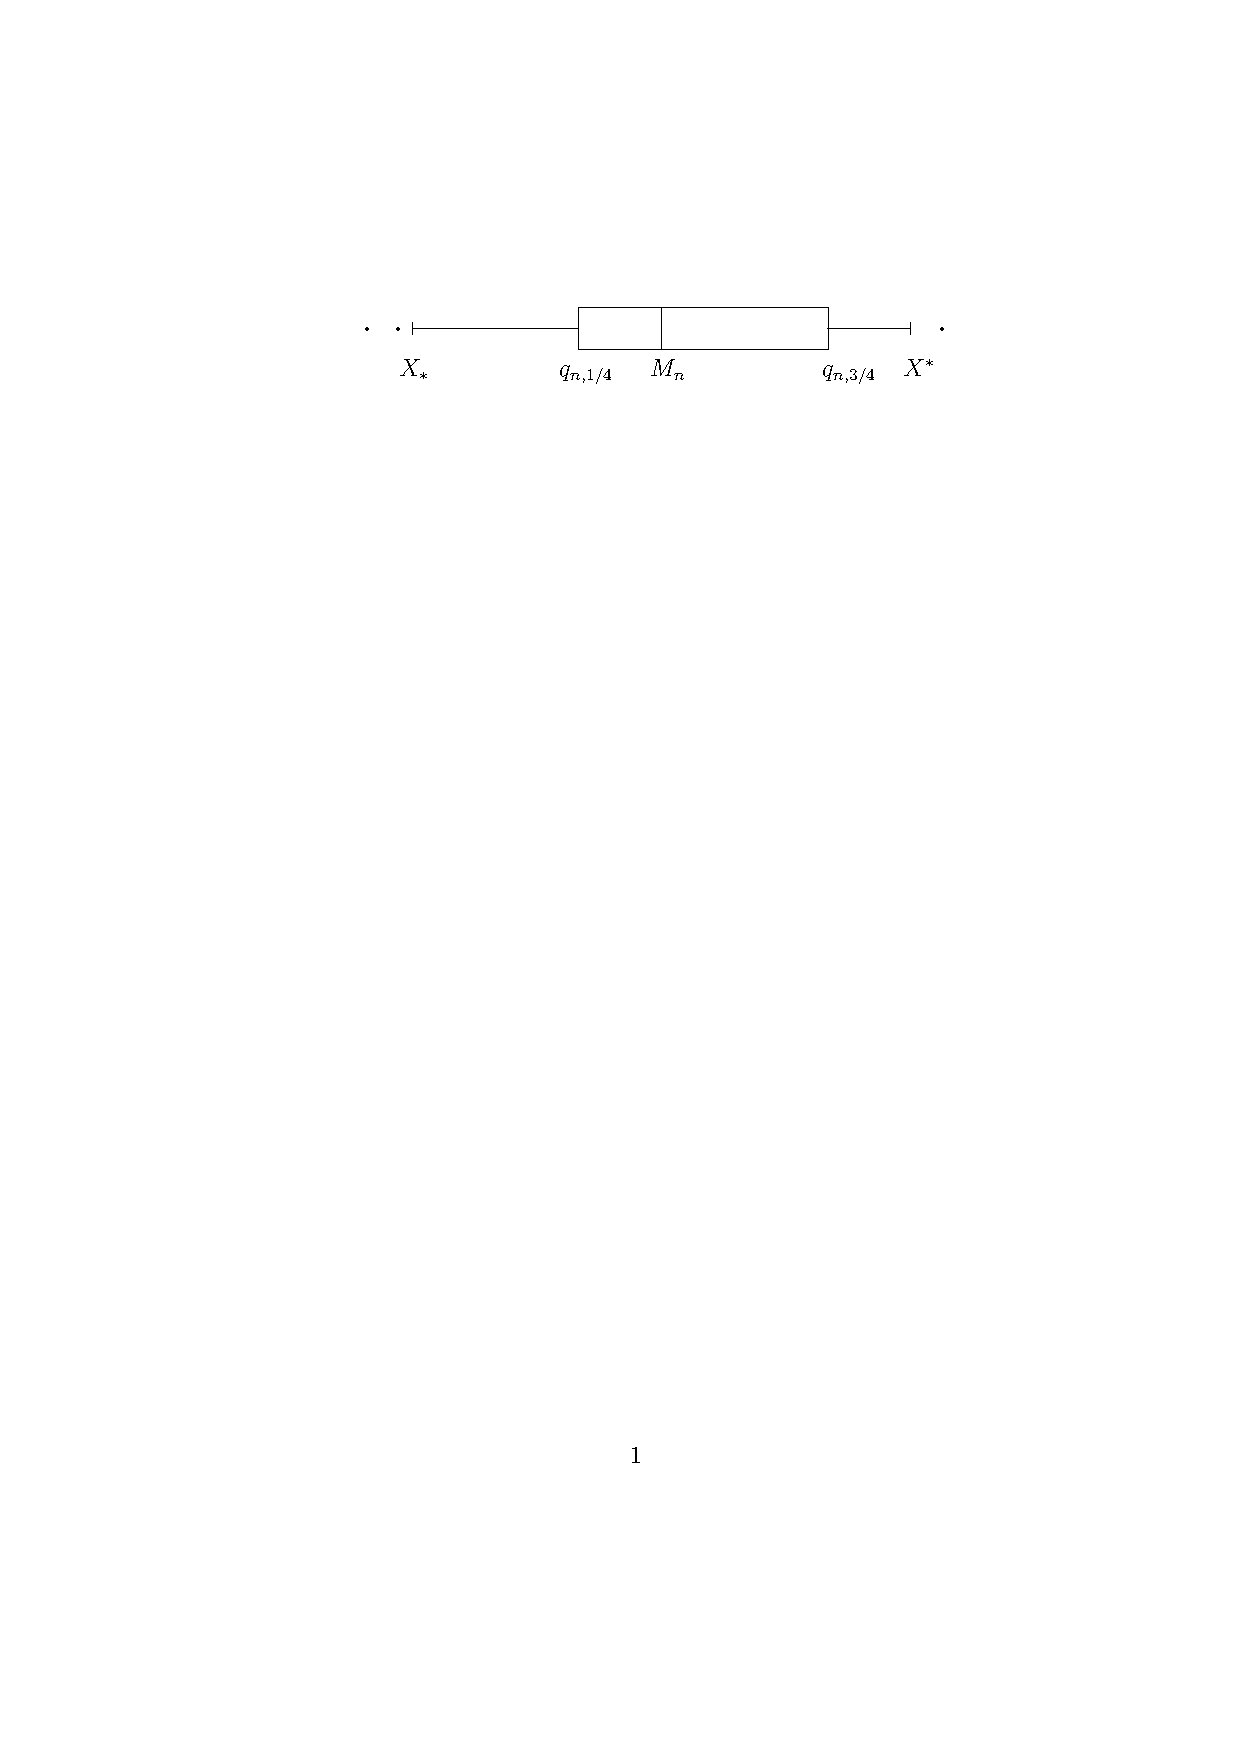
\includegraphics[height=1.3\textheight]{boxplot_def.pdf}
%\end{center}
    \begin{picture}(10,-70)
\put(120, -30){\framebox(120, 20)} \put(160,-30){\line(0,1){20}}
\put(120,-20){\line(-1,0){80}} \put(240,-20){\line(1,0){40}}
\put(40,-23){\line(0,1){6}} \put(280,-23){\line(0,1){6}}
\put(18,-20){\circle*{2}} \put(33,-20){\circle*{2}}
\put(295,-20){\circle*{2}}
\end{picture}

\vspace{1.0cm}

\noindent \hspace{32pt} $X_*$ \hspace{55pt} $\hat q_{n,1/4}$
\hspace{10pt} $M_n$  \hspace{58pt} $ \hat q_{n,3/4}$ \hspace{5pt}
$X^*$

\vspace{0.5cm}

$$
X_* = \min \{X_i : |X_i-\hat q_{n,1/4}| \le 1,5 {\mathcal I}_n\},
$$
$$
X^* = \max \{X_i : |X_i-\hat q_{n,3/4}| \le 1,5 {\mathcal I}_n\}.
$$
Intervalle interquartile:
$$
{\mathcal I}_n = \hat q_{n,3/4} - \hat q_{n,1/4}.
$$

\end{frame}

\begin{frame}
\begin{figure}
  \centering
  % Requires \usepackage{graphicx}
  \includegraphics[width=1.1\textwidth]{agedistribution.png}\\
  %\caption{}\label{}
\end{figure}
\end{frame}




\begin{frame}
\frametitle{Convergence  de l'estimateur par substitution}
\[
T(F)= h \left( \int_\rset g(x) dF(x) \right) \quad \text{et} \quad T(\hat{F}_n)= h \left( \int_\rset g(x) d \hat{F}_n(x) \right)
\]
\begin{theo}[Convergence]
 si $g,h:\R\rightarrow \R$, $h$
continue et $\E|g(X)|<\infty$, alors
$$
T(\widehat F_n) \plim T(F)
$$
\end{theo}
\end{frame}

\begin{frame}
\frametitle{Delta-méthode: cas scalaire}
\begin{theo}
Soit $\phi : \mathbb{D}_\phi \subset \rset \mapsto \rset$ une fonction définie sur un sous-ensemble ouvert de $\rset$ et différentiable au point $\mu$. Soit $(T_n)_{n \geq 0}$ une suite de v.a. à valeurs dans $\mathbb{D}_\phi$ et $(r_n)_{n \geq 0}$ une suite croissante telle que $\lim_{n \to \infty} r_n = \infty$. Si $r_n(T_n- \mu) \dlim T$, alors
$$
r_n \{ \phi(T_n) - \phi(\mu) \} \dlim \phi'(\mu) T \eqsp.
$$
\end{theo}
\end{frame}

\begin{frame}
\frametitle{Preuve}
\begin{itemize}
\item La fonction $\phi$ est différentiable au point $\mu$;
\[
\phi(t)= \phi(\mu) + \phi'(\mu) (t-\mu) + (t-\mu) \psi_\mu(t) \eqsp.
\]
\pause \item Donc,
\[
r_n \{ \phi(T_n) - \phi(\mu) \} = \phi'(\mu) r_n \{ T_n - \mu \} + r_n \{ T_n - \mu \} \psi_\mu(T_n) \eqsp.
\]
\pause \item Comme $\psi$ est continue en $\mu$, $T_n \plim \mu \, \Rightarrow \, \psi(T_n) \plim \psi(\mu)$.
\pause \item Comme $r_n( T_n - \mu) \dlim T$, on conclut par le Lemme de Slutsky.
\end{itemize}
\end{frame}

\begin{frame}
\frametitle{Vitesse de convergence de l'estimateur de substitution: Etape 1}
\[
T(F)= h \left( \int_\rset g(x) dF(x) \right) \quad \text{et} \quad T(\hat{F}_n)= h \left( \int_\rset g(x) d \hat{F}_n(x) \right)
\]
\begin{itemize}
\item \alert{TCL} :
$$\sqrt{n}\left(n^{-1}\sum_{i=1}^ng(X_i)-\int_{\R}g(x)dF(x)\right) \stackrel{d}{\rightarrow} {\mathcal N}\big(0,\mathrm{Var}\big[g(X)\big]\big),$$
où 
\begin{align*}
\text{Var}\big[g(X)\big]  &= \int_{\R}g(x)^2dF(x)-\big(\int_{\R}g(x)dF(x)\big)^2.
\end{align*}
\end{itemize}
\end{frame}

\begin{frame}
\frametitle{Vitesse de convergence de l'estimateur de substitution: Etape 2}
\[
T(F)= h \left( \int_\rset g(x) dF(x) \right) \quad \text{et} \quad T(\hat{F}_n)= h \left( \int_\rset g(x) d \hat{F}_n(x) \right)
\]
\begin{itemize}
\item \alert{TCL} :
$$\sqrt{n}\big(n^{-1}\sum_{i=1}^ng(X_i)-\int_{\R}g(x)dF(x)\big) \dlim \gauss\left(0,\mathrm{Var}\big[g(X)\big]\right),$$
\item \alert{Delta-méthode}
\[
\sqrt{n} \{ T(F_n) - T(F) \} \dlim \gauss\left(0, \{ h'(\PE[g(X)]) \}^2 \var[ g(X) ] \right)
\]
car si $Z \sim \gauss(0,\sigma^2)$, $a Z \sim \gauss(0, a^2 \sigma^2)$.
\end{itemize}
\end{frame}


\begin{frame}
\frametitle{Conclusion}
\begin{prop}
Si $\E[g(X)^2]<+\infty$ et $h$ continûment différentiable, alors
$$\sqrt{n}\big(T(\widehat F_n)-T(F)\big)\stackrel{d}{\rightarrow} \gauss\big(0,v(\alert{F})\big),
$$
où $v(\alert{F}) = h'\big(\E\big[g(X)\big]\big)^2\mathrm{Var}\big[g(X)\big]$.
\end{prop}
Pour construire un \alert{intervalle de confiance}, il faut encore remplacer $v(\alert{F})$ par $v(\widehat F_n)$.
\alert{On montre que} $v(\widehat F_n)\stackrel{\PP}{\rightarrow} v(F)$ et, via le lemme de Slutsky,
$$
\sqrt{n}\frac{T(\widehat F_n)-T(F)}{v(\widehat F_n)^{1/2}}\stackrel{d}{\rightarrow} {\mathcal N}\big(0,1\big).
$$
On \alert{en déduit} un intervalle de confiance asymptotique comme précédemment.
\end{frame}
\begin{frame}
\frametitle{Le cas de la dimension $d>1$}
\begin{itemize}
\item Il s'agit de fonctionnelles de la forme
$$T(F) = h\left(\int_{\R}g_1(x)dF(x),\ldots, \int_{\R}g_k(x)dF(x)\right)$$
où $h:\R^k\rightarrow \R$ continûment différentiable.
\item \alert{Exemple} : le coefficient d'asymétrie
$$T(F) = \frac{\int_{\R}\big(x-m(F)\big)^3dF(x)}{\sigma^{3/2}(F)},$$
$m(F)=$ moyenne de $F$, $\sigma^2(F) =$ variance de $F$.
\item \alert{Outil :} Version multidimensionnelle du TCL et de la \og méthode delta \fg{}.
\end{itemize}
\end{frame}

\begin{frame}
\frametitle{Méthode \og delta\fg{} multidimensionnelle}
\begin{itemize}
\item \alert{TCL multidimensionnel :}
$(\bX_n)_{n\ge 1}$ vecteurs aléatoires dans $\R^k$, i.i.d., de
moyenne ${\boldsymbol \mu} = \E[\bX_1]$ et de matrice de
variance-covariance $\Sigma =
\E\big[(\bX_1-\boldsymbol{\mu})(\bX_1-\boldsymbol{\mu})^T\big]$ bien
définie. Alors $\bar \bX_n=\tfrac{1}{n}\sum_{i = 1}^n\bX_i$
v\'erifie:
$$\sqrt{n}\big(\overline{\bX}_n-\boldsymbol{\mu}\big) \stackrel{d}{\rightarrow} {\mathcal N}\big(0,\Sigma\big).$$
%\end{itemize}
%\end{frame}
%\begin{frame}
%\begin{itemize}
\item \alert{Méthode \og delta\fg{} multidimensionnelle :} Si, de plus, $h : \R^k \rightarrow \R$ continûment différentiable, alors
$$\sqrt{n}\big(h(\overline{\bX}_n)-h(\boldsymbol{\mu})\big) \stackrel{d}{\rightarrow} {\mathcal N}\Big(0, \nabla h(\boldsymbol{\mu}) \Sigma \nabla h(\boldsymbol{\mu})^T\Big).$$
\end{itemize}
\end{frame}
\begin{frame}
\frametitle{Application : coefficient d'asymétrie}
\begin{itemize}
\item \alert{Coefficient d'asymétrie :} on a
$$T(F) = h\Big(\int_{\R} xdF(x),\int_{\R} x^2 dF(x), \int_{\R} x^3 dF(x)\Big)$$ avec
$$h(\alpha,\beta,\gamma) = \frac{\gamma-3\alpha \beta+2\alpha^3}{(\beta-\alpha^2)^{3/2}}.$$
$$T(\widehat F_n) = h\Big(\tfrac{1}{n}\sum_{i = 1}^n X_i, \tfrac{1}{n}\sum_{i = 1}^n X_i^2,\tfrac{1}{n}\sum_{i = 1}^n X_i^3\Big).$$
\item On applique le TCL multidimensionnel avec $\bX_i = (X_i,X_i^2,X_i^3)^T$ et $\boldsymbol{\mu} = \big(\int_{\R} xdF(x),\int_{\R} x^2 dF(x),\int_{\R} x^3 dF(x)\big)^T$, puis la méthode \og delta\fg{} avec $h$.
\end{itemize}
\end{frame}
\begin{frame}
\frametitle{Limites de l'approche empirique} L'estimation de $T(F)$
par $T(\widehat F_n)$ n'est pas toujours \alert{possible}:
%
%
\begin{itemize}
\item La fonctionnelle $F \leadsto T(F)$ n'est pas \og régulière\fg{},
\item La paramétrisation $F \leadsto T(F)$ ne donne \alert{pas} lieu à une \alert{forme analytique simple}.
%et ne s'étudie pas à force d'arguments standard basés sur la loi des grands nombres et le TCL
$\rightarrow$ autres approches.
\end{itemize}
%
\underline{Exemple}. \alert{Hypothèse} : $F$ admet une densité
$f$ par rapport à le mesure de Lebesgue, \alert{continue} ($=$ presque-partout à une fonction continue $f$).
$$T(F) = f(x_0),\;\;x_0\in \R \,\;\text{(donné)}.$$
On ne \alert{peut pas prendre} comme estimateur $\widehat
F_n'(x_0)$ car $\widehat F_n$ n'est pas diff\'erentiable (constante
par morceaux...)

\end{frame}

\begin{frame}
\frametitle{Limites de l'approche empirique} L'estimation de $T(F)$
par $T(\widehat F_n)$ n'est pas toujours \alert{souhaitable} :
\begin{itemize}
\item
Souvent on dispose d'information \alert{a priori}
supplémentaire : $F$ appartient à une sous-classe \alert{
particulière} de distributions, et il y a des choix plus judicieux
que l'estimateur par substitution.
\end{itemize}
\end{frame}

%\begin{frame}
%\frametitle{Exemple 2 : information supplémentaire}
%\end{frame}
%\begin{frame}
%\frametitle{Exemple 3 : paramétrisation non-standard}
%\end{frame}

\begin{frame}
\frametitle{Conclusion}
\begin{itemize}
\item \alert{L'approche empirique}, basée sur $\widehat F_n$ permet d'estimer une distribution inconnue $F$ ou une fonctionnelle $T(F)\in \R$ à partir d'un $n$-échantillon, mais
\begin{itemize}
\item reste très générale, pas toujours adaptée.
%(cas de fonctionnelles irrégulières ou difficiles à paramétriser en $F$)
\item restreinte à la situation d'un $n$-échantillon.
%\item reste très générale...
%(en particulier, n'incorpore pas d'information supplémentaire de modélisation)
\end{itemize}
\item Formalisation de la notion \alert{d'expérience statistique }
\begin{itemize}
\item incorporation d'information de modélisation \alert{supplémentaire}.
\item construction de méthodes d'estimation -- de décision -- \alert{systématiques}.
\item comparaison et \alert{optimalité} des méthodes.
\end{itemize}
\end{itemize}
\end{frame}

\section{Modélisation statistique}
\subsection{Expérience statistique}
\begin{frame}
\frametitle{Expérience statistique} Consiste à identifier:
\begin{itemize}
\item \alert{Des observations}
$${\tt x}_1,{\tt x}_2,\ldots, {\tt x}_n$$
\alert{considérées} comme des \alert{réalisations} de variables aléatoires $Z = (X_1,\ldots, X_n)$ de loi $\PP^Z$.
\item \alert{Une famille de lois}
$$\left\{\PP_\theta,\,\theta \in \Theta\right\}.$$
\item \alert{Une problématique} "estimer" le paramètre $\theta$ ou bien prendre une décision sur une propriété relative à $\theta$ (test).
\end{itemize}
\end{frame}

\begin{frame}
\frametitle{Expérience statistique}
\begin{itemize}
\item Approche g\'en\'erale empirique:
\begin{itemize}
\item $\theta=F$, $\Theta$ est l'ensemble de
toutes les lois (s'il s'agit de l'estimation de $F$);
\item $\theta=F$, $\Theta$ est l'ensemble de
toutes les lois v\'erifiant une hypoth\`ese tr\`es g\'en\'erale, par
exemple, la bornitude d'un moment (s'il s'agit de l'estimation de
$T(F)$).
\end{itemize}
\item Approche param\'etrique: \alert{on suppose} que $F$ appartient \`a une
\alert{famille de lois connue} index\'ee par un param\`etre
$\theta$ de dimension finie: $\theta\in \Theta \subset \R^d$.
\begin{itemize}
\item \underline{Exemple}: $\Theta = \R$,
$$ X_i= \theta +\xi_i, \quad i=1,\dots,n,$$
$\xi_i$ v.a. i.i.d. de densit\'e \alert{connue} $f$ sur $\R$
et $\E(X_i)=\theta$.

\underline{Question}: en utilisant cette information
suppl\'ementaire, peut-on construire un estimateur plus performant
que l'estimateur $\bar X_n$ bas\'e sur l'approche empirique?
\end{itemize}
%
\end{itemize}
\end{frame}


\begin{frame}
\frametitle{Expérience statistique}
\begin{itemize}
\item En \'ecrivant
$$ X_i= \theta +\xi_i, \quad i=1,\dots,n,$$
$\xi_i$ v.a. i.i.d. de densit\'e \alert{connue} $f$, nous
pr\'ecisons la forme de la loi $\PP_{\theta}$ de
$(X_1,\dots,X_n)$:
$$\PP_\theta\big[A\big] = \int_A
\left(\prod_{i=1}^n f(x_i-\theta)\right) dx_1\ldots dx_n,
$$
pour tout $A\in {\mathcal B}(\R^n)$.
\end{itemize}
\end{frame}


\begin{frame}
\frametitle{Expérience statistique}
\begin{df}
Une expérience (un modèle) statistique ${\mathcal E}$ est le triplet
$${\mathcal E} = \left(\mathfrak{Z}, {\mathcal Z}, \,\big\{\PP_\theta, \theta \in \Theta\big\}\right),$$
avec
\begin{itemize}
\item $\big(\mathfrak{Z}, {\mathcal Z}\big)$ espace mesurable (souvent
$(\R^n,{\mathcal B}(\R^n))$),
\item $\{\PP_\theta,\,\theta \in \Theta\}$ famille de probabilités définies \alert{simultanément} sur le même espace  $\big(\mathfrak{Z}, {\mathcal Z}\big)$,
\item $\theta$ est le \alert{paramètre (inconnu)}, et $\Theta$ est \alert{ l'ensemble des paramètres}.
\end{itemize}
\end{df}
\end{frame}


%\begin{frame}
%\frametitle{Description (mathématique) d'une expérience statistique}
%\begin{itemize}
%\item Deux points de vue \alert{équivalents} et (parfois ?) source de confusion :
%\begin{itemize}
%\item Expérience \underline{engendrée par une observation}.
%\item Expérience \underline{canonique}
%\end{itemize}
%\item \alert{Traitement sur un exemple} : on \og observe \fg{} $X_1,\ldots, X_n$ i.i.d. de loi exponentielle de paramètre $\theta >0$.
%\end{itemize}
%\end{frame}


\begin{frame}
\frametitle{Experience engendrée par ($X_1,\ldots, X_n$)}
\begin{itemize}
\item On observe
$$Z = (X_1,\ldots, X_n), \quad\quad X_i= \theta + \xi_i,$$
$\xi_i$ v.a. i.i.d. de densit\'e \alert{connue} $f$.
\item La famille de lois $\big\{\PP_\theta^n,\theta \in \Theta  =
\R\big\}$ est définie sur $\mathfrak{Z}=\R^n$ par
$$\PP_\theta^n\big[A\big] = \int_A
\left(\prod_{i=1}^n f(x_i-\theta)\right) dx_1\ldots dx_n,
$$
pour $A\in{\mathcal Z}= {\mathcal B}(\R^n)$ (et $\PP^Z$ est l'une
des $\PP_\theta^n$).
\item Expérience \alert{engendrée par l'observation $Z$} :
$${\mathcal E}^n = \big(\R^n,{\mathcal B}(\R^n),\big\{\PP_\theta^n,\,\theta \in \Theta\big\}\big).$$
\end{itemize}
\end{frame}

%\begin{frame}
%\frametitle{Expérience -- observation canonique}
%\begin{itemize}
%\item Si on part de ${\mathcal E}^n = \big(\R^n,{\mathcal B}(\R^n),\big\{\PP_\theta^n,\,\theta \in \Theta\big\}\big)$, \alert{il n'y a plus d'observation !} On a perdu la structure (trop lourde) de tout l'espace $\big(\Omega, {\mathcal F}, \PP\big)$ et des observations $X_1,\ldots, X_n$.
%\item On peut \alert{toujours \og fabriquer \fg{} une observation} $Z$ dont l'expérience engendrée soit ${\mathcal E}^n$.
%Il suffit de poser
%$$\big(\Omega, {\mathcal F}\big):=\big(\mathfrak{Z}, {\mathcal Z}\big) \stackrel{\text{ici}}{=}\big(\R^n,{\mathcal B}(\R^n)\big),$$
%et
%$$Z(\omega) = \omega\;\;\;\text{observation canonique}.$$
%\end{itemize}
%\end{frame}

\begin{frame}
\frametitle{Expérience (mod\`ele) paramétrique, non-paramétrique}
\begin{itemize}
\item Si $\Theta$ est  un sous-ensemble
de $\R^d$ : \alert{expérience (=mod\`ele) paramétrique}.
\item Sinon (par exemple si le paramètre $\theta$ est un élément d'un espace fonctionnel) : \alert{expérience (=mod\`ele) non-paramétrique}.
\end{itemize}
\end{frame}

\subsection{Expériences dominées}
\begin{frame}
\frametitle{Expériences dominées}
\begin{itemize}
\item On fait une hypothèse minimale de \og complexité \fg{} sur le modèle statistique. \alert{But} : ramener l'étude de la famille
$$\{\PP_\theta,\,\theta \in \Theta\}$$
à l'étude d'une famille de fonctions
$$\left\{z \in \mathfrak{Z} \leadsto f(\theta,z) \in \R_+,\,\theta \in \Theta\right\}.$$
\item Via la notion de \alert{domination}. Si $\mu,\nu$ sont deux mesures $\sigma$-finies sur $\mathfrak{Z}$, alors $\mu$ \alert{domine} $\nu$ (notation $\nu \ll \mu$) si
$$\mu\big[A\big]=0 \Rightarrow \nu\big[A\big]=0.$$
\end{itemize}
\end{frame}
\begin{frame}
\frametitle{Théorème de Radon-Nikodym}
\begin{theo}
Si $\nu \ll \mu$, il existe une fonction positive
$$z \leadsto  p(z) \stackrel{\text{notation}}{=} \frac{d\nu}{d\mu}(z),$$ définie $\mu-$p.p., $\mu-$ intégrable, telle que
$$\nu\big[A\big] = \int_{A}p(z) \mu(dz) = \int_{A}\tfrac{d\nu}{d\mu}(z)\mu(dz),\;\;A \in {\mathcal Z}.$$
%\underline{Notation} :
%$$p(z)=\frac{d\nu}{d\mu}(z),\;\;\text{densité de}\;\nu\;\text{par rapport à}\;\mu.$$
\end{theo}
\end{frame}
\begin{frame}
\frametitle{Expérience dominée}
\begin{df}
Une expérience statistique ${\mathcal E} = \big(\mathfrak{Z}, {\mathcal Z}, \big\{\PP_\theta, \theta \in \Theta\big\}\big)$ est \alert{dominée} par la mesure $\sigma$-finie $\mu$ définie sur $\mathfrak{Z}$ si
$$\forall \theta \in \Theta : \PP_\theta \ll \mu.$$
\end{df}
On appelle \alert{densités} de la famille $\{\PP_\theta,\theta \in \Theta\}$ la famille de fonctions (définies $\mu-$ p.p.)
$$z\leadsto \frac{d\PP_\theta}{d\mu}(z),\;z\in \mathfrak{Z},\;\theta \in \Theta.$$
\end{frame}




\subsection{Modèle de densité}

\begin{frame}
\frametitle{Modèle de densité (paramétrique)}
\begin{itemize}
\item On observe un $n$-échantillon de v.a.r. $X_1,\ldots, X_n$.
\item La loi des $X_i$ appartient à
$\{\PP_\theta,\,\theta \in \Theta\}$, famille de \alert{probabilités sur $\R$}, \alert{dominée} par une mesure ($\sigma$-finie) $\mu(dx)$ sur $\R$.
\item La loi de $(X_1,\ldots,X_n)$ s'écrit
\begin{align*}
\PP_\theta^n(dx_1\cdots dx_n) & = \PP_\theta(dx_1)\otimes \cdots \otimes \PP_\theta(dx_n) \\
& \ll  \mu(dx_1)\otimes \cdots \otimes \mu(dx_n) \\
& \stackrel{\text{\alert{notation}}}{=} \mu^n(dx_1\cdots dx_n)
\end{align*}
%\item \alert{L'expérience statistique} engendrée par $(X_1,\ldots, X_n)$ s'écrit :
%$${\mathcal E}^n = \Big(\R^n, {\mathcal B}(\R^n), \big\{\PP_\theta^n,\theta \in \Theta\big\}\Big),\;\;\alert{\Theta \subset \R^d}.$$
\end{itemize}
\end{frame}

\begin{frame}
\frametitle{Modèle de densité (paramétrique)}
\begin{itemize}
\item \alert{Densité du modèle} : on part de
$$f(\theta,x)=\frac{d\PP_\theta}{d\mu}(x),\;\;x\in \R$$
et
$$\frac{d\PP_\theta^n}{d\mu^{n}}(x_1,\ldots, x_n) = \prod_{i = 1}^n f(\theta,x_i),\;\;x_1,\ldots, X_n \in \R.$$
\item  \alert{L'expérience statistique} engendrée par $(X_1,\ldots, X_n)$ s'écrit :
$${\mathcal E}^n = \Big(\R^n, {\mathcal B}(\R^n), \big\{\PP_\theta^n,\theta \in \Theta\big\}\Big),\;\;\alert{\Theta \subset \R^d}.$$
\end{itemize}
\end{frame}

\begin{frame}
\frametitle{Exemple 1 : modèle de densité gaussienne univariée}
\begin{itemize}
\item $X_i\sim {\mathcal N}(m,\sigma^2)$,
avec
$$\theta = (m,\sigma^2) \in \Theta = \R\times \R_+\setminus\{0\}.$$
\begin{align*}
\PP_\theta(dx) = f(\theta,x)dx & =\frac{1}{\sqrt{2\pi \sigma^2}}\exp\Big(-\frac{(x-m)^2}{2\sigma^2}\Big)dx \\
& \ll \mu(dx)=dx.
\end{align*}
\item Puis
\begin{align*}
\frac{d\PP_{\tco{\theta}}^n}{d\mu^n}(x_1,\ldots, x_n) & = \prod_{i = 1}^n f(\tco{\theta},x_i) \\
& =(2\pi \tco{\sigma^2})^{-n/2}\exp\big(-\frac{1}{2\tco{\sigma^2}}\sum_{i = 1}^n (x_i-\tco{m})^2\big),
\end{align*}
avec $x_1,\ldots,x_n \in \R$.
\end{itemize}
\end{frame}

\begin{frame}
\frametitle{Exemple 2 :  modèle de Bernoulli}
\begin{itemize}
\item $X_i \sim \text{Bernoulli}(\theta)$, avec $\theta \in \Theta = [0,1]$.
\begin{align*}
\PP_\theta(dx)& = (1-\theta)\, \delta_{0}(dx) + \theta\, \delta_1(dx) \\
& \ll \mu(dx) = \delta_0(dx)+\delta_1(dx)\;\;\text{(mesure de comptage)}.
\end{align*}
\item Puis
$$\boxed{\frac{d\PP_{\tco{\theta}}}{d\mu}(x) = (1-\alert{\theta})\,1_{\{x=0\}}+\alert{\theta}\,1_{\{x=1\}} = \alert{\theta}^x(1-\alert{\theta})^{1-x}}$$
\alert{avec $x\in \{0,1\}$}, et
$$\frac{d\PP_\theta^n}{d\mu^n}(x_1,\cdots, x_n) = \prod_{i = 1}^n \theta^{x_i}(1-\theta)^{1-x_i},$$
\alert{avec $x_i \in \{0,1\}$}.
\end{itemize}
\end{frame}

\begin{frame}
\frametitle{Exemple 3 : temps de panne arrêtés}
\begin{itemize}
\item On observe $X_1,\ldots, X_n$, où $X_i = Y_i \wedge T$, avec $Y_i$ \alert{lois exponentielles} de paramètre $\theta$ et $T$ \alert{temps fixe} (censure).
\item Cas 1 : $T=\infty$ (pas de censure). Alors  $\theta \in \Theta = \R_+\setminus \{0\}$ et
$$\PP_\theta(dx) = \theta \exp(-\theta x)1_{\{x \geq 0\}}dx \ll \mu(dx) = dx$$
et
$$
\frac{d\PP_{\tco{\theta}}^n}{d\mu^n}(x_1,\ldots,x_n) = \tco{\theta}^n \exp\left(-\tco{\theta} \sum_{i = 1}^n x_i\right),
$$
\alert{avec $x_i \in \R_+$} .
\item Cas 2 : \alert{Comment s'écrit le modèle} dans la cas où $T<\infty$ (présence de censure) ? Comment choisir $\mu$ ?
\end{itemize}
\end{frame}





\end{document}
